% Chapter 3
\chapter{Contributions} % Main chapter title

\label{Chapter3} % For referencing the chapter elsewhere, use \ref{Chapter3} 

%----------------------------------------------------------------------------------------

\section{Voting Classifier}
A voting classifier was extracted from the scikit-learn library and modified to handle classification in a streaming setting. There were two voting schemes previously implemented; the first was a "hard" vote, which uses the predicted class labels for majority voting; and a "soft" vote, which selects the label with the highest probability average. 
\textit{Big blurb on voting classifiers}

%----------------------------------------------------------------------------------------

\section{FHDDMS}

Additionally, this thesis builds upon my colleague's, Ali Pesaranghader, work \parencite{pesaranghader2016fast} in which he proposes a concept drift detection algorithm that uses a sliding window storing whether or not the classifier predicted the class properly. To detect the drift, the author uses Hoeffding's inequality to detect when a significant change occurs between the maximum probability of correct predictions and the most recent probability of correct predictions. The authors found that FHDDMS was able to detect a drift with a smaller delay and greater accuracy when compared to the state-of-the-art.

\textit{Bigger blurb on how FHDDMS works}

%----------------------------------------------------------------------------------------

\section{Improvements to voting classifier for concept drift}

As previously stated, the scikit-learn voting classifier implements two voting strategies: the first being "soft" voting and the second being "hard" voting. The former calculates the probability that one or many tuples belong to a given class label. The latter performs a majority voting, meaning that the class label with the highest number of votes will be chosen.
The "soft" voting strategy also requires that all classifiers in the voting ensemble be capable of outputting a probability associated to its class label prediction.

We implemented one additional voting scheme similar to the "soft" scheme in that it requires its classifiers to output a probability or confidence in the class label prediction. Our method uses a logistic function with a sigmoid curve function to weigh the probability, centered around seventy five percent (75\%) confidence.
Logistic functions have the following equation
\begin{equation}
    f(x)=\frac{L}{1+e^{-k(x-x_0)}}\\ 
    \label{eq:logistic_function}
\end{equation}
where \textit{e} is the natural logarithm base, \textit{$x_0$} is the x-value of the sigmoid's midpoint, \textit{L} is the curve's maximum value, and \textit{k} is the steepness of the curve.

The logistic function that we used, uses the following values for the variables listed above. $x_0=0.75$, $L=1$, and $k=11$. These values were selected based on the resulting graph for values of x between zero and one ([0;1]), which allowed us to assign almost no weight to predictions with a probability of under forty percent (40\%), and give more weight to predictions with a probability of over seventy five percent (75\%).

Our proposed voting strategy therefore computes the sum of this logistic function using the prediction of each classifier for each class label. See the following equation:
\begin{equation}
    \sum_{i=0}^{c} \frac{\frac{1}{1+e^{-11(p_i(X)-0.75)}}}{\frac{1}{1+e^{-11(0.25)}}}\\ 
    \label{eq:logistic_sum}
\end{equation}
where $c$ is the number of classifiers in the voting ensemble and $p_i(X)$ is the probability of classifier $i$ predicting that the tuple belongs to class X. We then divide by the maximum value for $p_i(X)$ to ensure that our sum covers all values from 0 to 1.

Another weighting equation is proposed to determine if it is possible to achieve similar results by using a different function that resembles the logistic sigmoid function presented above while being less computationally intensive.
The weighting function is seen in equation \ref{eq:sin_weight_fn} and the sum is seen in equation \ref{eq:sin_sum}. The plot of equation \ref{eq:sin_weight_fn} is almost identical to the plot of \ref{eq:logistic_function}, with a maximum difference of approximately 0.0183 over [0, 1].
\begin{equation}
    f(x)=sin^8(\frac{x*\pi}{2})
    \label{eq:sin_weight_fn}
\end{equation}
\begin{equation}
\sum_{i=0}^{c} sin^8(\frac{p_i(X)*\pi}{2})
    \label{eq:sin_sum}
\end{equation}
The sums presented in equations \ref{eq:logistic_sum} and \ref{eq:sin_sum} are calculated for each class label. The class label with the highest sum is thereafter selected as the winner in the vote, and we hope proves to be more accurate based on the importance of the weight of the predicted class probability.

%----------------------------------------------------------------------------------------

\section{Hybrid sliding-tumbling windows}
One of many issues in data stream data mining is execution time, in the sense that our algorithm must learn faster than tuples can arrive. In our case, we want to determine if we can delay training of some classifiers in our VE, and how it affects execution time and classifying performance, as well as drift detection.

We propose the following algorithm, also seen in figure \ref{alg:sliding_tumbling_windows}, titled \textit{Sliding-Tumbling windows for training the VE}.
Let the number of tuples (single tuple or chunk) used in the interleaved test-then-train loop iterations be \textit{number\_of\_tuples}, and let \textit{number\_of\_classifiers} be the number of classifiers in the voting ensemble (VE). The VE will have a window size of \textit{number\_of\_tuples}*\textit{number\_of\_classifiers}. At every iteration of the interleaved test-then-train loop, we will append the new tuples to the VE's window and train a single classifier in the VE. For the next \textit{number\_of\_classifiers - 1} iterations, we will train the remaining \textit{number\_of\_classifiers - 1} classifiers in the ensemble so that from the point of view of the VE, we are training and testing using sliding windows but from the point of each c classifier, we are training them using tumbling windows.

While not used for the same purpose, my colleague Sarah D'Ettore used the same sliding batches to improve CDC-Stream in her thesis \citep{d2016fine}. Figure \ref{fig:sliding_tumbling_windows}, taken from my colleagues' thesis, shows how the algorithm works for three (3) classifiers in the ensemble with a batch size of one (1) and a window size of three (3). Each classifier will only learn from the same coloured batch; meaning that at time \textit{t}, only a single classifier has enough tuples to learn from, but the others will learn at time \textit{t+1} and finally at time \textit{t+2}. Each classifier will be learning from what essentially is a tumbling window, from their point of view, just not all from the same one.

The motivation for this technique is to determine if we can spend less execution time training the classifiers and to investigate how progressively delaying training of some of classifiers in the VE affects concept drift detection and classification performance while also hopefully reducing execution time.

\begin{algorithm}
\KwIn{X, y}
\KwResult{at least one classifier in the VE was trained}
\eIf {classifiers never been trained yet}{
    classifierToFit = classifierList[index]\\
    index = index+1 modulo numberOfClassifiers\\
    classifierToFit.partialTrain(X, y)
}{
    \For{$classifier \in classifierList$}{
        classifier.partialTrain(X, y)
    }
}
\caption{Sliding-Tumbling windows for training the VE\label{alg:sliding_tumbling_windows}}
\end{algorithm}

\begin{figure}
  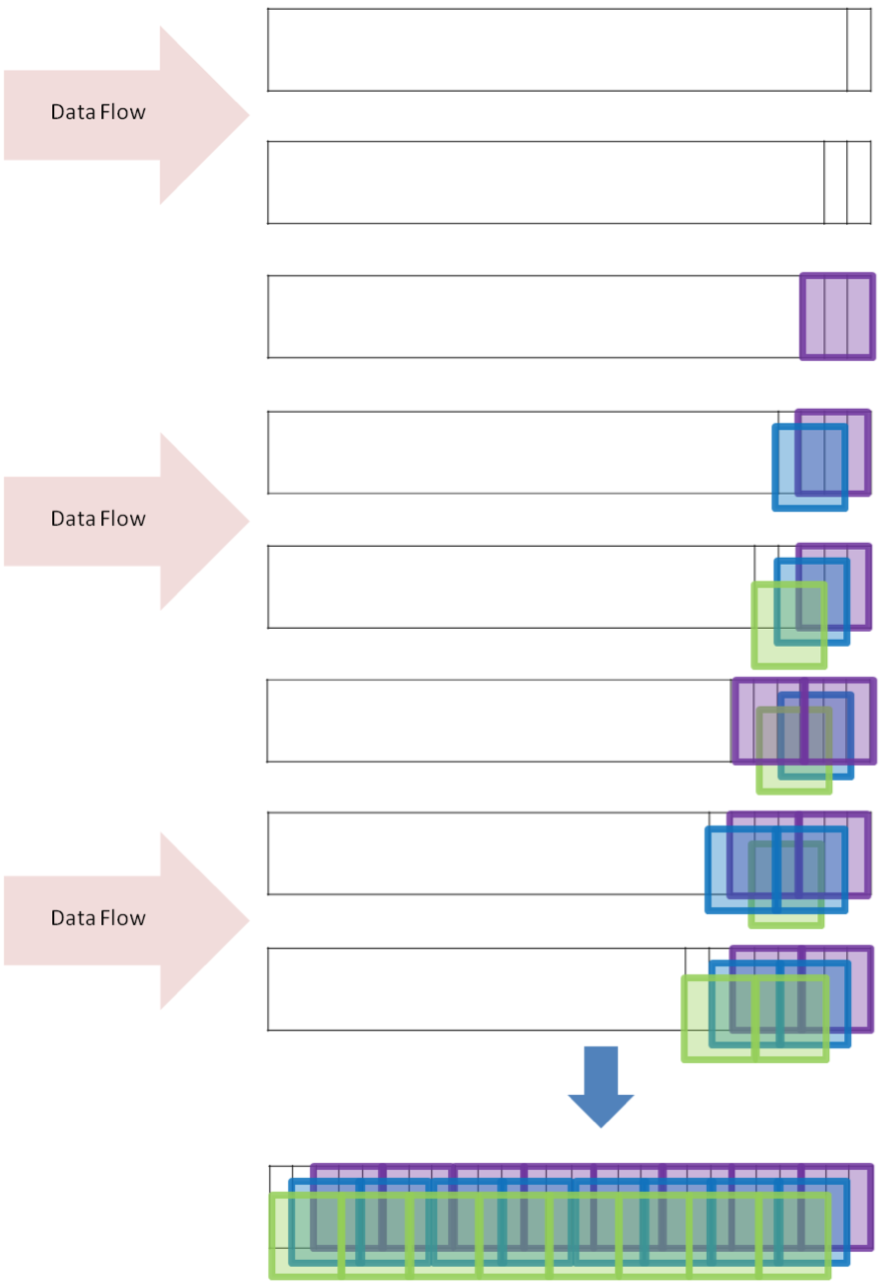
\includegraphics[width=\linewidth]{./Figures/sliding_tumbling_windows.png}
  \caption{Sliding Tumbling windows.}
  \label{fig:sliding_tumbling_windows}
\end{figure}



%----------------------------------------------------------------------------------------

\section{Improvements to voting classifier to reduce dependency on ground truth}

The interleaved test-then-train methodology in a data streaming setting has a rather large flaw: we are assuming that we obtain the ground truth immediately after testing. This means that we assume that the ground truth is always available in a fraction of a second after testing our models. For the large majority of cases, this approach is not realistic in a real world setting.

Therefore, we wanted to determine if we could re-use the idea behind self-training in an offline setting to reduce our dependency on the ground truth in the online streaming setting for the interleaved test-then-train method. We propose an approach that is, as previously stated, similar to self-training in that we use the classifier's prediction, and not ground truth, when training.

However, using only the predictions to train our model in an online setting is a recipe for disaster. The known cons to using self-training in an offline setting is that it can reinforce and classification errors; it is therefore a logical conclusion to assume that we will encounter the same risks in porting this idea to a streaming setting.

Given the restriction of limiting reinforcing misclassification errors, we want to determine at what ratio of predictions to ground truth our voting ensemble's accuracy would decline and by how much.

The algorithm behind this idea is very straightforward: it consists in duplicating the ground truth array, and replacing at random a particular fraction of values with the actual prediction from the classifier.

%----------------------------------------------------------------------------------------

\section{Improvements to FHDDMS to remove dependency on ground truth}

Along the same lines of the previous section, the drift detection algorithm proposed by my colleague Dr. Pesaranghader in \cite{pesaranghader2016fast}, \textit{FHDDMS}, relies on immediate knowledge of the ground truth after testing and after training. The drift detection mechanism in FHDDMS relies on storing, in a sliding window, whether or not the classifier accurately predicted the class. This method only applies to a select few domains where ground truth can be available almost instantly after the tuples are generated. For the large majority of domains, this method simply isn't applicable.

It is for that reason that we have set out to study how much ground truth can be omitted in the case of FHDDMS to reduce or remove its dependency on immediate knowledge of the ground truth to detect drifts in an online streaming setting.

In order to do so, we have opted to modify FHDDMS to run inside of the voting ensemble, with one sliding window per classifier in the ensemble. In each sliding window, we store not whether the classifier accurately predicted the class label, but rather if that sliding window's classifier voted for the class label that won the ensemble vote.

It is our hope that we can achieve similar results for drift detection speed while maintaining good classification accuracy.

%----------------------------------------------------------------------------------------

\section{Summary}

%----------------------------------------------------------------------------------------